\documentclass[12pt,twoside]{article}
\usepackage[utf8]{inputenc}
\usepackage{blindtext,changepage,caption,subcaption,graphicx,booktabs,pgfplots,multirow,appendix,mathtools,fancyhdr,pst-plot,floatrow,amsmath,cases,apacite,natbib,caption,tikz,rotating,subcaption,lmodern,graphicx,outlines,amsmath,amsfonts,amssymb,subcaption,mwe, hyperref,sectsty, afterpage}
\usepackage[en-US]{datetime2}
% ------ % Setting style
\hypersetup{
	pdftex,
	pdfauthor={Nurlan Jahangirli and friends},     % author
	colorlinks=true,       % false: boxed links; true: colored links
	linkcolor=red,          % color of internal links
	citecolor=black,        % color of links to bibliography
	urlcolor=blue           % color of external links
}
\sectionfont{\fontsize{16}{0}\selectfont}
\newcommand\blankpage{%
	\null
	\thispagestyle{empty}%
	\addtocounter{page}{-1}%
	\newpage}
\definecolor{ChadGreen}{rgb}{0,.4,0}    % Dark Green
\definecolor{ChadBlue}{rgb}{.1,.1,.5}  
\newcommand{\runningheads}[2]{
	\chead[\color{ChadGreen}{\uppercase {\footnotesize #1}}]  % Author page header
	{\color{ChadGreen}{\uppercase {\footnotesize #2}}}  % Short title
} 

\usepackage{xcolor}
\usepackage[width=1\textwidth,font={small, sf},labelfont={color=ChadBlue,bf, sf},
labelsep=colon, format=plain]{caption}

\makeatother
\floatsetup[table]{capposition=top}
\floatsetup[figure]{capposition=top}
\usepackage[left=2.5cm,right=2.5cm,top=3cm,bottom=3cm]{geometry}
\usepackage{setspace}
\doublespacing
% This is how to control linespacing using setspace
% (\singlespacing or doublespacing just call this command)
%\setstretch{1.4}
%% Setting up page headers
\pagestyle{fancy}
\rhead[]{\thepage}
\lhead[\thepage]{}
\cfoot[]{} 
\renewcommand{\headrulewidth}{0pt}
% Make hyperlinks jump more accurately
\makeatletter
\newcommand\org@hypertarget{}
\let\org@hypertarget\hypertarget
\renewcommand\hypertarget[2]{%
	\Hy@raisedlink{\org@hypertarget{#1}{}}#2%
} \makeatother 
% Spacing in Tables and Figures
%\renewcommand{\tabcolsep}{1pt}   % space between columns
\renewcommand{\arraystretch}{1.5} % space between rows
\addtolength{\textfloatsep}{0pt} % space between floats and text
\addtolength{\abovecaptionskip}{0pt} % space above caption
\addtolength{\belowcaptionskip}{.15in} % space below caption

\let\LaTeXtitle\title
\renewcommand{\title}[1]{\LaTeXtitle{\color{ChadBlue}{\LARGE #1}}}
\renewcommand{\abstractname}{\color{ChadBlue}Abstract}
% \renewcommand{\figurename}{\color{ChadBlue}Figure}
% \renewcommand{\tablename}{\color{ChadBlue}Table}
% Add a period *only* after Section and *only* in title, not cross ref
% April 2017
\makeatletter
\renewcommand{\@seccntformat}[1]{%
	\csname the#1\endcsname% Print sectional counter
	\ifnum\pdfstrcmp{#1}{section}=0 .\fi% If \section, print .
	\quad% Space between number and title
}
\makeatother

% ------- % Setting the graphicspath
\graphicspath{{../../}} 

% ------ % Title page
\urldef{\njahangirliWeb}\url{http://development-review.org/}	\urldef{\njahangirliEmail}\url{nurlan.jahangirli@monash.edu}
\newtheorem{proposition}{Proposition}
\title{A paper}
\author{Nurlan Jahangirli\thanks{Monash U \njahangirliEmail} \\ Monash University}
\date{\color{ChadGreen} \large First draft: t-1 \\ This revision: \today \\ COMMENTS WELCOME}
\runningheads{Nurlan Jahangirli}{A Paper}
	
	
	\begin{document}
\maketitle


% -----------------------------------------------
% 	ABSTRACT
% -----------------------------------------------

\begin{abstract}
	 %\noindent  \input{./sections/abstract.tex}
\end{abstract}
\vspace{1cm}
{\small
	\noindent \textit{Keywords}:  \\
	\textit{JEL codes}: 
}
\thispagestyle{empty}
\newpage
\setcounter{page}{1}



% -----------------------------------------------
% 	BODY
% -----------------------------------------------

%\input{./sections/intro.tex}
%\input{./sections/theory.tex}
%\input{./sections/estimation.tex}
%\input{./sections/discussion.tex}

% -----------------------------------------------
% 	REFERENCES
% -----------------------------------------------
	
\bibliographystyle{chicago}
\bibliography{../../ProjectA.bib}

\newpage
\clearpage

\begin{center} \Large \textbf{Appendix -- For Online Publication} \end{center}
\appendix
\numberwithin{equation}{section}
\numberwithin{figure}{section}
\numberwithin{table}{section}

%\input{./sections/appendix_theory}
%\input{./sections/appendix_data.tex}
%\input{./sections/appendix_empirics.tex}



\begin{figure}
	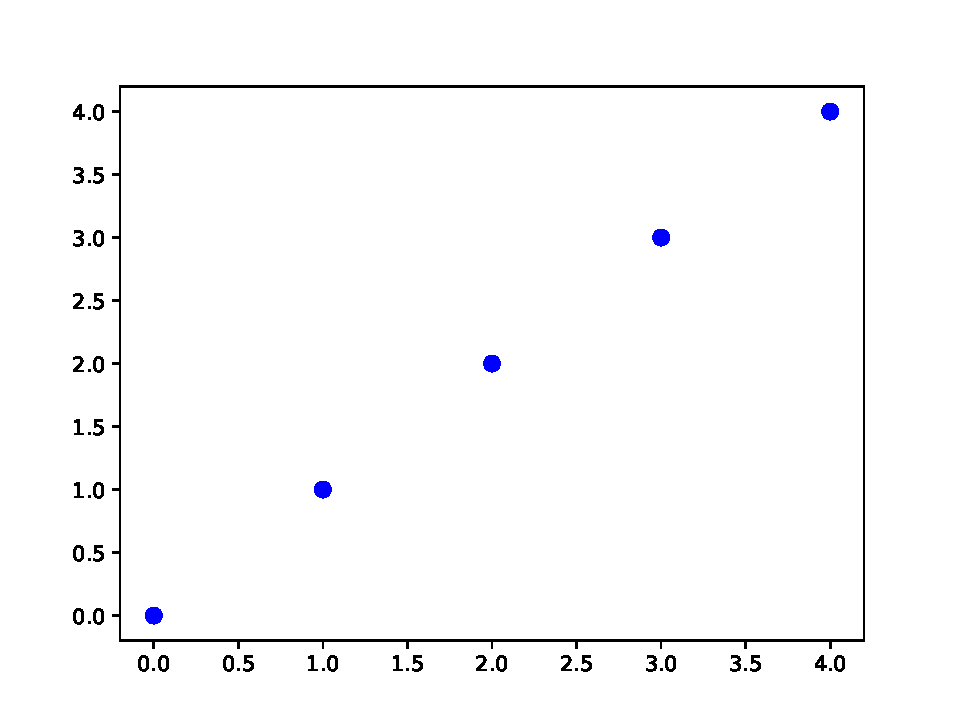
\includegraphics[width=\textwidth]{figures/chart.pdf}
\caption{Example figure. \label{fig:example}}
\end{figure}	



\end{document}

